% Template for Elsevier CRC journal article
% version 1.1-5p dated 18 January 2011

% This file (c) 2010-2011 Elsevier Ltd.  Modifications may be freely made,
% provided the edited file is saved under a different name

% This file contains modifications for Procedia Computer Science
% but may easily be adapted to other journals

% Changes since version 1.0
% - elsarticle class option changed from 1p to 3p (to better reflect CRC layout)
% - this version uses option 5p for larger-format journals (text area 24.1 x 18.4 cm)

%-----------------------------------------------------------------------------------

%% This template uses the elsarticle.cls document class and the extension package ecrc.sty
%% For full documentation on usage of elsarticle.cls, consult the documentation "elsdoc.pdf"
%% Further resources available at http://www.elsevier.com/latex

%-----------------------------------------------------------------------------------

%%%%%%%%%%%%%%%%%%%%%%%%%%%%%%%%%%%%%%%%%%%%%%
%%%%%%%%%%%%%%%%%%%%%%%%%%%%%%%%%%%%%%%%%%%%%%
%%                                          %%
%% Important note on usage                  %%
%% -----------------------                  %%
%% This file must be compiled with PDFLaTeX %%
%% Using standard LaTeX will not work!      %%
%%                                          %%
%%%%%%%%%%%%%%%%%%%%%%%%%%%%%%%%%%%%%%%%%%%%%%
%%%%%%%%%%%%%%%%%%%%%%%%%%%%%%%%%%%%%%%%%%%%%%

%% The '5p' and 'times' class options of elsarticle are used for Elsevier CRC
\documentclass[5p,times,authoryear]{elsarticle}

%% The `ecrc' package must be called to make the CRC functionality available
%% ecrc_SCI es el paquete ecrc de Elsevier con modificaciones para la revista RIAI a su vez modificadas para las Actas del Simposio de Control Inteligente.

\usepackage{ecrc_SCI}

%% The ecrc package defines commands needed for running heads and logos.
%% For running heads, you can set the journal name, the volume, the starting page and the authors

%%%%%%%%%%%%%%%%%%%%%%%%%%%%%%%%% Añadido por Secretaría RIAI / CEA
\usepackage[utf8]{inputenc}
\usepackage[brazilian]{babel}     % Idioma
\addto\captionsspanish{%
\def\tablename{Tabla}%
}
%\usepackage[latin1]{inputenc}   % Lengua latina
\usepackage{amsmath}            % Para las referencias a ecuaciones con \eqref
                                % Para igualar las columnas de la última página
%\usepackage{hyperref}           % Para hipervínculos dentro del PDF
%%%%%%%%%%%%%%%%%%%%%%%%%%%%%%%%%%%%%%%%%%%%%%%%%%%%%%%


%% set the volume if you know. Otherwise `00'
%% Establecer la edición del Simposio
\volume{XVI}

%% set the starting page if not 1
\firstpage{1}

%% Give the name of the journal
\journalname{Actas del Simposio de Control Inteligente}

%% Give the author list to appear in the running head
%% Example \runauth{C.V. Radhakrishnan et al.}
\runauth{Primer autor et al.}


%% Give the abbreviation of the Journal. Contast the Publisher if in doubt what this is.
\jid{SCI}

%% Give a short journal name for the dummy logo (if needed)
\jnltitlelogo{}

%% Hereafter the template follows `elsarticle'.
%% For more details see the existing template files elsarticle-template-harv.tex and elsarticle-template-num.tex.

%% Elsevier CRC generally uses a numbered reference style
%% For this, the conventions of elsarticle-template-num.tex should be followed (included below)
%% If using BibTeX, use the style file elsarticle-num.bst

%% End of ecrc-specific commands
%%%%%%%%%%%%%%%%%%%%%%%%%%%%%%%%%%%%%%%%%%%%%%%%%%%%%%%%%%%%%%%%%%%%%%%%%%

%% The amssymb package provides various useful mathematical symbols
\usepackage{amssymb}
%% The amsthm package provides extended theorem environments
%% \usepackage{amsthm}

%% The lineno packages adds line numbers. Start line numbering with
%% \begin{linenumbers}, end it with \end{linenumbers}. Or switch it on
%% for the whole article with \linenumbers after \end{frontmatter}.
%% \usepackage{lineno}

%% natbib.sty is loaded by default. However, natbib options can be
%% provided with \biboptions{...} command. Following options are
%% valid:

%%   round  -  round parentheses are used (default)
%%   square -  square brackets are used   [option]
%%   curly  -  curly braces are used      {option}
%%   angle  -  angle brackets are used    <option>
%%   semicolon  -  multiple citations separated by semi-colon
%%   colon  - same as semicolon, an earlier confusion
%%   comma  -  separated by comma
%%   numbers-  selects numerical citations
%%   super  -  numerical citations as superscripts
%%   sort   -  sorts multiple citations according to order in ref. list
%%   sort&compress   -  like sort, but also compresses numerical citations
%%   compress - compresses without sorting
%%
%% \biboptions{comma,round}

% \biboptions{}

% if you have landscape tables
\usepackage[figuresright]{rotating}

% put your own definitions here:
%   \newcommand{\cZ}{\cal{Z}}
%   \newtheorem{def}{Definition}[section]
%   ...

% add words to TeX's hyphenation exception list
%\hyphenation{author another created financial paper re-commend-ed Post-Script}

% para poder introducir varias figuras que ocupen el ancho de las dos columnas.
\usepackage{subfigure}

% declarations for front matter

\begin{document}

\begin{frontmatter}

%% Title, authors and addresses

%% use the tnoteref command within \title for footnotes;
%% use the tnotetext command for the associated footnote;

%% use the fnref command within \author or \address for footnotes;
%% use the fntext command for the associated footnote;

%% use the corref command within \author for corresponding author footnotes;
%% use the cortext command for the associated footnote;
%% use the ead command for the email address,
%% and the form \ead[url] for the home page:
%%
%% \title{Title\tnoteref{label1}}
%% \tnotetext[label1]{}
%% \author{Name\corref{cor1}\fnref{label2}}
%% \ead{email address}
%% \ead[url]{home page}
%% \fntext[label2]{}
%% \cortext[cor1]{}
%% \address{Address\fnref{label3}}
%% \fntext[label3]{}

%\dochead{Cabecera artaculo}
% Use \dochead if there is an article header, e.g. \dochead{Short communication}

\title{Preparación de artículos para el SCI: Use este tipo para el título del artículo}


%% use optional labels to link authors explicitly to addresses:
%% \author[label1,label2]{<author name>}
%% \address[label1]{<address>}
%% \address[label2]{<address>}

\author[First]{Primer A. Autor\corref{cor1}\fnref{label2}}
\ead{autor@cea-ifac.es}
\ead[url]{www.cea-ifac.es}

\author[Second]{Segundo B. Autor, Jr.}
\ead{autor2@cea-ifac.es}
\ead[url]{www2.cea-ifac.es}

\author[Third]{Tercer C. Autor}
\ead{autor3@cea-ifac.es}

\fntext[label2]{Nota al pie para el autor 1}
\cortext[cor1]{Autor en correspondencia.}


\address[First]{Comité Español de Automática, Parc Tecnologic de Barcelona, Edifici U, C/ Llorens i Artigas, 4-6, 08028 Barcelona, España. }
\address[Second]{Departamento de Automática, Ingeniería Electrónica e Informática, Universidad Politécnica de Madrid,  C/ José Gutiérrez Abascal, na2, 28006, Madrid,  España.}
\address[Third]{Departamento de Ingeniería de Sistemas y Automática,  Universitat Politècnica de Valencia, Camino de Vera, na14, 46022, Valencia, España.}

\begin{abstract}
 Text of abstract
Estas instrucciones constituyen una guía para la preparación de artículos para las actas de los simposios de Control Inteligente. Utilice este documento como un conjunto de instrucciones. También puede usarse como una ``plantilla'' para preparar su manuscrito. Para las directrices de envío, siga las instrucciones del sistema de envío de artículos de la página web del correspondiente simposio. \emph{Copyright {\copyright} XXXX CEA. Publicado por Universidad de Xxxx Xxxx. Todos los derechos reservados.}
\end{abstract}

\begin{keyword}
 keywords here, in the form: keyword \sep keyword

palabra 1 \sep palabra 2 \sep 5-10 palabras clave (tomadas de la lista del sitio web de IFAC).

\end{keyword}

\end{frontmatter}


\section{Introducción}
Estas instrucciones constituyen una guía para la preparación de artículos para las actas de los simposios de Control Inteligente. Utilice este documento como un conjunto de instrucciones. Puede usar este documento como una ``plantilla'' para preparar su manuscrito en Latex. Para las directrices de envío, siga las instrucciones del sistema de envío de artículos de la pagina web del correspondiente simposio. {\bf{\emph {No cambie el tamaño de las fuentes o espaciado de línea para introducir mas texto en un número limitado de paginas}}}.  Utilice cursiva para enfatizar; no subraye.

\subsection{Una subsección de ejemplo.}
Bifurcación: Trazado del máximo local de $x$ con una disminución de amortiguamiento $a$ (Fig.~\ref{fig1}).

Para insertar imágenes en \emph{Word}, posicione el cursor en el punto de inserción y o bien utilice Insertar | Imagen | Desde Fichero o copie la imagen al portapapeles de Windows y entonces use Editar | Pegado especial | Imagen (con ``Flotar sobre el texto'' deseleccionado).

Los organizadores del simposio no realizarán ninguna operación de formateado final a su artículo. Su documento debe estar ``listo para filmar''. El número límite de hojas para el documento es de doce. {\bf Por favor, no modifique los márgenes. Si esta creando el documento usted mismo, tenga en cuenta los márgenes listados en la Tabla 1.}

\section{Procedimiento para el envío de artículos}

Recuerde que las actas de los simposios están consideradas como un \emph{Camera Ready Copy Journal (CRC)}. Esto implica que los autores son responsables de aplicar el formato correspondiente a sus contribuciones. Desde la coordinación del simposio no se ejecutará ninguna acción de formateo a los artículos. A continuación vemos unas subsecciones.

\subsection{Fase de revisión}

Por favor, use este documento como una ``plantilla'' para preparar su documento. Para las directrices de envío, siga las instrucciones del sistema de envío de artículos en la web del simposio.

Dado que el limite de paginas es de doce, es mejor preparar el envío inicial en el formato listo para filmar, de tal manera que tenga una buena estimación de la longitud de hojas. Adicionalmente, el esfuerzo requerido para el envío de la versión final será, de esta manera, mínimo.

\subsection{Fase final}

Se supone que los autores tendrán en cuenta rigurosamente los márgenes. En caso de no ser así se le pedirá que reenvíe el documento para que así lo cumpla, retrasando de esta manera la preparación de los contenidos de las actas. \citep{Baker1963}, \citep{Baker1963a}

\subsection{Inserción de tablas}
La tabla ocupa el ancho de la columna porque el entorno \emph{tabular} lleva el asterisco. Se puede usar \emph{table}* para confeccionar una tabla que se expanda sobre la dos columnas del texto. Y por supuesto combinar ambos efectos \citep{Charlie1966}.


\begin{table}[htbp]
  \caption{Preferencias para el diseño de un controlador}
   \label{extremos45}
  \begin{tabular*}{\hsize}{lrrrrr}
\hline
    & $g_i^1$ & $g_i^2$ & $g_i^3$ & $g_i^4$ & $g_i^5$ \\
    \hline
$Re(\lambda)_{max}$ & -0.01  & -0.005 & -0.001 & -0.0005 & -0.0001 \\
$u_{max}$& 0.85 & 0.90 & 1 & 1.5 & 2  \\
$t_{est}^{max}$& 14 & 16 & 18 & 21 & 25 \\
$noise_{max}$& 0.5 & 0.9 & 1.2 & 1.4 & 1.5  \\
$u_{nom}$& 0.5 & 0.7 & 1  & 1.5 & 2  \\
$t_{est}^{nom}$& 10 & 11 & 12 & 14 & 15 \\
\hline
  \end{tabular*}
\end{table}


\begin{table*}
\centering
\caption{Comparación de las especificaciones para cada diseño del sistema. }
\label{tabladeseables}
\begin{tabular}{lcccccc}   \hline
Controlador  & $Re(\lambda)_{max}$  & $u_{max}$ & $t_{est}^{max}$ & $noise_{max}$ & $u_{nom}$ & $t_{est}^{nom}$  \\ \hline
B23 & INA & INA & INA & INA & AD & AIND \\
M23 & AD & AD & AD & T & AD & AIND \\
PPGA23 & \textbf{AD} & \textbf{AD}& \textbf{AD}&\textbf{AD} &\textbf{AD} & \textbf{AD}\\
 \hline
 W34 & AD & AD & D & T & AD & IND \\
 M34 & AD & AD & D & AD & AD & AD \\
 \textbf{PPGA23}* & \textbf{AD} & \textbf{AD} & \textbf{AD} & \textbf{AD} & \textbf{AD} & \textbf{AD} \\
 \textbf{PPGA34} & \textbf{AD} & \textbf{AD} & \textbf{AD} & \textbf{AD} & \textbf{AD} & \textbf{AD} \\
  \hline
J45 & AD & IND & AD & IND & AD & AD \\
M45 & AD & AD & IND & T & AD & IND \\
\textbf{PPGA23}**& \textbf{D} & \textbf{AD} & \textbf{D} & \textbf{T} & \textbf{AD} & \textbf{D} \\
\textbf{PPGA34}**& \textbf{AD} & \textbf{AD} & \textbf{D} & \textbf{D} & \textbf{AD} & \textbf{D}  \\
\textbf{PPGA45} & \textbf{AD} & \textbf{AD} & \textbf{AD} & \textbf{AD} & \textbf{AD} & \textbf{D} \\
 \hline
\end{tabular}
\end{table*}

Es muy importante mantener estos márgenes. Son necesarios para poner información de la revista y los números de pagina.

\subsection{Figuras y creación del PDF}
Todas las figuras deben estar incrustadas en el documento. Cuando incluya una imagen, asegúrese de insertar la imagen real en lugar de un enlace a su computador local. En la medida de lo posible, utilice las herramientas de conversión a PDF estándares Adobe Acrobat o Ghostscript que dan los mejores resultados. \textbf{Es importante que todas las fuentes estén incrustadas/subconjunto en el PDF resultante.}

Al compilar utilizando PDFLatex, se pueden insertar figuras en png (logo grupo CI), jpg (figura \ref{fig2}) o pdf (figura \ref{fig3}). Si tiene figuras en eps conviértalas a pdf previamente o bien haga uso del paquete epstopdf.


\begin{figure}
\centering
  % El fichero es un eps y se convierte automáticamente a pdf con eps2pdf package
  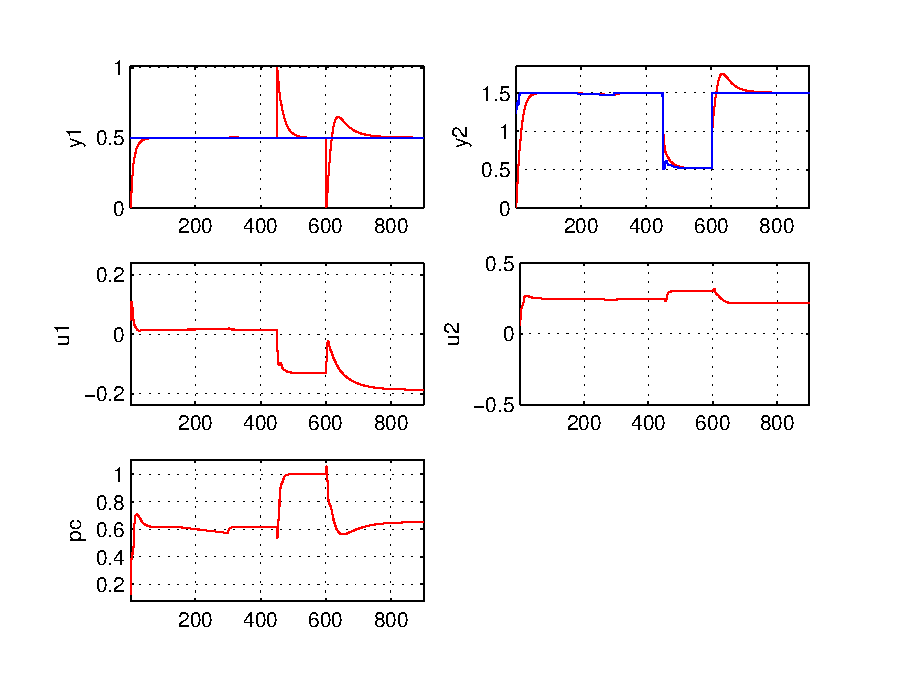
\includegraphics[width=7cm]{Figuras/figuraeps}\\
  \caption{Título de la figura 1. La figura es un fichero eps y gracias al paquete epstopdf se convierte automáticamente a pdf. También se podría convertir previamente la figura con un programa como Adobe Distiller}\label{fig1}
\end{figure}

\begin{figure}
\centering
   Se pueden incluir figuras jpeg al compilar con PDFLatex
  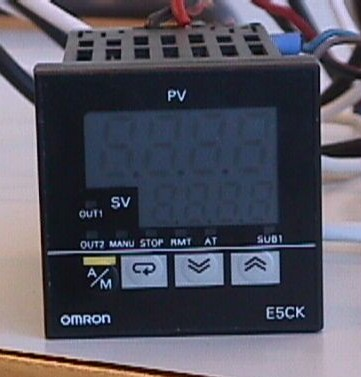
\includegraphics[width=3cm]{Figuras/figurajpeg}\\
  \caption{Título de la figura 2}\label{fig2}
\end{figure}


\section{Unidades}

Use el Sistema Internacional como unidades primarias. Se pueden usar otras unidades como unidades secundarias (entre paréntesis). Esto se aplica a artículos sobre almacenamiento de datos. Por ejemplo, escriba ``$15 Gb/cm^2$'' ($100 Gb/in^2$). Se considera una excepción cuando las unidades inglesas se usan como identificadores comerciales, como unidad de disco de 3.5 pulgadas. Evite mezclar unidades del Sistema Internacional con el Sistema Cegesimal, tales como corriente en amperios y campo magnético en  oersteds. Esto a menudo lleva a confusión porque las ecuaciones no son dimensionalmente equiparables. Si debe usar unidades mezcladas, especifique claramente las unidades para cada cantidad  en la ecuación. \citep{Able1945}

La unidad en el Sistema Internacional para la fuerza del campo magnético H es A/m. Sin embargo, si desea utilizar unidades de $T$, o bien refiérase a densidad de flujo magnético $B$ o fuerza del campo magnético simbolizado como $\mu_0 H$. Utilice el punto centrado para separar unidades compuestas,  es decir, $A\cdot m^2$.

\section{Consejos útiles}

\subsection{Mas sobre figuras y tablas}

Las etiquetas de los ejes de las figuras son a menudo fuentes de confusión. Utilice palabras en lugar de símbolos. Como ejemplo, escriba la cantidad ``Magnetización,'' o ``Magnetización M,'' no solo ``M.'' Ponga las unidades entre paréntesis. No etiquete los ejes únicamente con unidades. Como en la Fig. 1, por ejemplo, escriba ``Magnetización (A/m)'' o ``Magnetización (A $\cdot$ m$^{-1}$),'' no solo ``A/m'' No etiquete los ejes con una relación de cantidades y unidades. Por ejemplo, escriba ``Temperatura (K),'' no ``Temperatura/K.''

Los multiplicadores pueden ser especialmente fuente de confusión. Escriba``Magnetización (kA/m)'' o ``Magnetización ($10^3$ A/m).'' No escriba ``Magnetización (A/m) $\times$ 1000'' porque el lector no sabría si la etiqueta del eje superior en la Fig. 1 es 16000 A/m o 0.016 A/m. Las etiquetas de las figuras deben ser legibles, aproximadamente de 8 a 12 puntos.

\subsection{Referencias} % ATENCION: usar \citep en lugar de \cite para ajustarse al formato de RIAI.

La lista de referencias debe ser ordenada alfabéticamente de acuerdo con el primer autor, con las siguientes líneas justificadas con la sangría correspondiente. Si existen diferentes publicaciones del mismo autor(es), estas deberán ser listadas en el orden del año de publicación. Si hay más de un artículo del mismo autor en la misma fecha, etiquételas como a,b, etc. (Sanchez et al., 2000a, b). Por favor, fíjese que todas las referencias \citep{Garcia2008} listadas en este apartado deben ser citadas directamente en el cuerpo del texto \citep{Garcia2007}, \citep{Dog1958}, \citep{Keohane1958}.

\begin{figure}
\centering
  % Requires \usepackage{graphicx}
  % Se pueden incluir figuras pdf al compilar con PDFLatex
  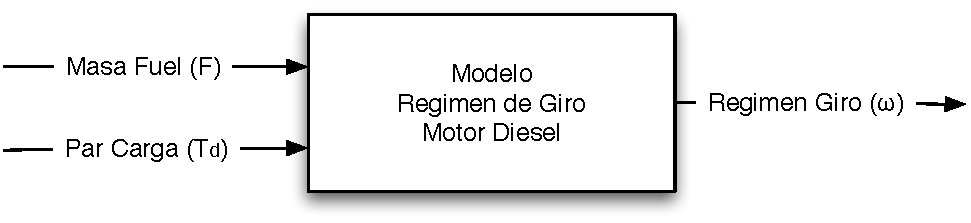
\includegraphics[width=7cm]{Figuras/figurapdf}\\
  \caption{Título de la figura 3}\label{fig3}
\end{figure}

Por favor, tenga en cuenta que las referencias al final de este documento cumplen con el estilo anteriormente mencionado. Los artículos que no hayan sido publicados deben ser citados como ``no publicado.'' Ponga en mayúscula únicamente la primera palabra del título, excepto el caso de nombres propios y símbolos de elementos.

Si esta utilizando LaTeX, puede procesar una base de datos de bibliografía externa o insertarla directamente en la sección de referencias. Las notas al pie de pagina se deben evitar en la medida de lo posible.

\subsection{Abreviaciones y acrónimos}

Defina las abreviaciones y acrónimos la primera vez que se usan en el texto, incluso después de que hayan sido definidos en el resumen. Abreviaciones tales como IFAC, SI, ac, y dc no necesitan ser definidas. Abreviaciones que incorporen periodos no deben tener espacios: escriba ``C.N.R.S.,'' no ``C. N. R. S.'' No utilice abreviaciones en el título salvo que sea inevitable (por ejemplo, ``SCI'' en el título de este artículo).

\section{Más sobre figuras}

Con el entorno \emph{figure*} se puede conseguir que una figura ocupe las dos columnas (ver figura \ref{mifigura}). Con el paquete \emph{subfigure} conseguimos una figura completa a partir de varios ficheros (como las subfiguras \ref{subfig1} y \ref{subfig2}).

\begin{figure*}[tb]
\centering
\subfigure[Título Subfigura 11]{
   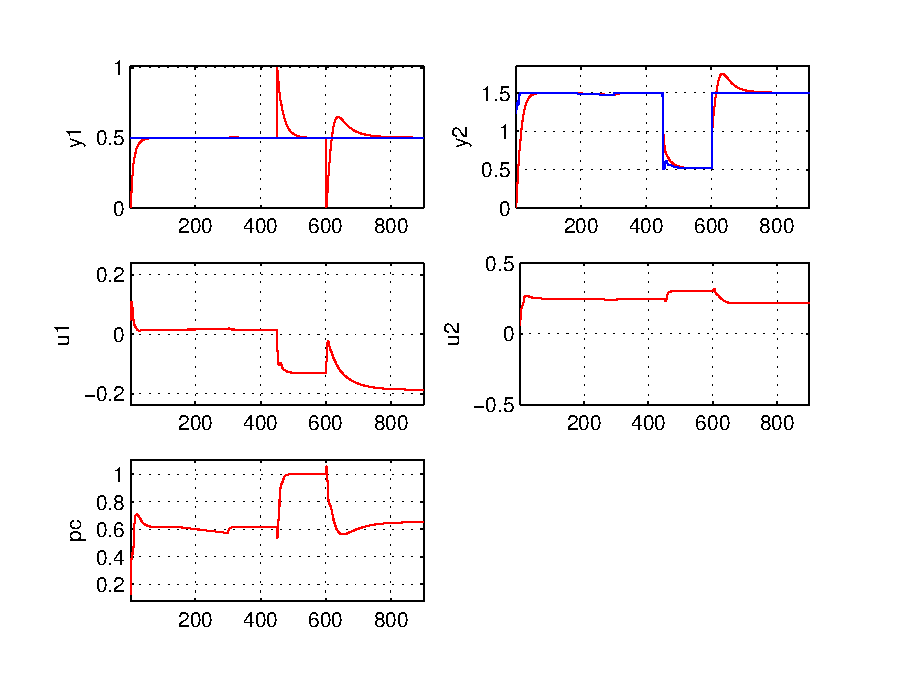
\includegraphics[scale =0.5] {Figuras/figuraeps}
   \label{subfig1}
 }
 \subfigure[Título Subfigura 2]{
   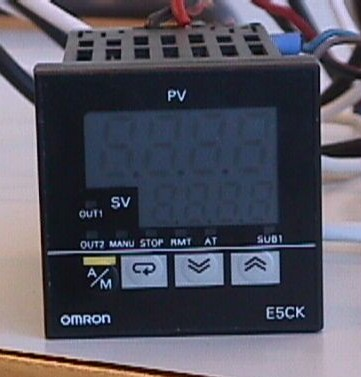
\includegraphics[scale =0.35] {Figuras/figurajpeg}
   \label{subfig2}
 }

\label{mifigura}
\caption{Título global para la figura.}
\end{figure*}

\subsection{Ecuaciones}

Numere las ecuaciones consecutivamente con números de ecuaciones entre paréntesis justificado al margen derecho, como en \eqref{e2}. Primero use el editor de ecuaciones para crear la ecuación. Después seleccione el estilo ``Equation''. Presione la tecla de tabulador y escriba el número de ecuación entre paréntesis. Para hacer sus ecuaciones más compactas, puede usar el solidus ( / ), la función exp, o los exponentes apropiados. Utilice paréntesis para evitar ambigüedades en los denominadores. Ponga signos de puntuación en las ecuaciones cuando formen parte de una frase, como en

\begin{equation} \label{e2}
\begin{array}{ll}
\int_0^{r_2} & F (r, \varphi ) dr d\varphi = [\sigma r_2 / (2 \mu_0 )] \\
& \cdot \int_0^{\inf} exp(-\lambda |z_j - z_i |) \lambda^{-1} J_1 (\lambda  r_2 ) J_0 (\lambda r_i ) d\lambda
\end{array}
\end{equation}

Asegúrese de que los símbolos de su ecuación han sido definidos antes de que la ecuación aparezca o inmediatamente después. Ponga en cursiva los símbolos (T podría referirse a la temperatura, pero T es la unidad tesla). Refiérase a ``(1),'' no ``Ec. (1)'' o ``ecuación (1),'' excepto al principio de la frase: ``La ecuación (1) es ....''

\subsection{Otras recomendaciones}

Utilice un espacio tras los periodos y dos puntos. Evite utilizar participios, tales como, ``Utilizando (1), se calcula el potencial.'' [No esta claro quién o qué usa (1).] En su lugar escriba ``El potencial fue calculado empleando (1),'' o ``Empleando (1), se calcula el potencial.''

\section{Conclusión}

Una sección de conclusiones no es necesaria. Sin embargo, las conclusiones pueden revisar los puntos mas importantes de un artículo, pero no debe replicarse el resumen en las conclusiones. Las conclusiones pueden tratar sobre la importancia del trabajo realizado o sugerir aplicaciones o trabajos futuros.

Repetido. Una sección de conclusiones no es necesaria. Sin embargo, las conclusiones pueden revisar los puntos mas importantes de un artículo, pero no debe replicarse el resumen en las conclusiones. Las conclusiones pueden tratar sobre la importancia del trabajo realizado o sugerir aplicaciones o trabajos futuros.

Repetido. Una sección de conclusiones no es necesaria. Sin embargo, las conclusiones pueden revisar los puntos mas importantes de un artículo, pero no debe replicarse el resumen en las conclusiones. Las conclusiones pueden tratar sobre la importancia del trabajo realizado o sugerir aplicaciones o trabajos futuros.

%%%%%%%%%%%%%%%%%%%%%%%%%%%%%%%%%%%%%%%%%%%%%%%%%%%%%%%%%%%%%%%%%%%%%%%%%%%%%%%%%%%%%%%%%%
\section*{Agradecimientos}

Este trabajo ha sido realizado parcialmente gracias al apoyo de la Agencia Nacional (los agradecimientos de financiación y apoyos han de ser incluidos aquí).



%% References with BibTeX database:

\bibliographystyle{elsarticle-harv}
\bibliography{sci2020}


\appendix
\section{Primer apéndice}    
Este texto está repetido. Si utiliza Word, use o bien Microsoft Editor de Ecuaciones o MathType  para las ecuaciones de su artaculo (Insertar | Objeto | Crear Nuevo | Microsoft Editor de Ecuaciones o Ecuación MathType).
No debe seleccionar la opción ``Flotar'' sobre el texto. Por supuesto, LaTeX gestiona las ecuaciones a través de macros pre-programadas.

\section{Segundo apéndice}

Este texto está repetido. Use el Sistema Internacional como unidades primarias. Se pueden usar otras unidades como unidades secundarias (entre paréntesis). Esto se aplica a artículos sobre almacenamiento de datos. Por ejemplo, escriba ``$15 Gb/cm^2$'' ($100 Gb/in^2$). Se considera una excepción cuando las unidades inglesas se usan como identificadores comerciales, como unidad de disco de 3.5 pulgadas. Evite mezclar unidades del Sistema Internacional con el Sistema Cegesimal, tales como corriente en amperios y campo magnético en  oersteds. Esto a menudo lleva a confusión porque las ecuaciones no son dimensionalmente equiparables. Si debe usar unidades mezcladas, especifique claramente las unidades para cada cantidad  en la ecuación.

La unidad en el Sistema Internacional para la fuerza del campo magnético H es A/m. Sin embargo, si desea utilizar unidades de $T$, o bien refiérase a densidad de flujo magnético $B$ o fuerza del campo magnético simbolizado como $\mu_0 H$. Utilice el punto centrado para separar unidades compuestas,  es decir, $A\cdot m^2$.

\section{Tercer apéndice}

\subsection{Más sobre figuras y tablas}

Este texto está repetido. Las etiquetas de los ejes de las figuras son a menudo fuentes de confusión. Utilice palabras en lugar de símbolos. Como ejemplo, escriba la cantidad ``Magnetización,'' o ``Magnetización M,'' no salo ``M.'' Ponga las unidades entre paréntesis. No etiquete los ejes únicamente con unidades. Como en la Fig. 1, por ejemplo, escriba ``Magnetización (A/m)'' o ``Magnetización (A $\cdot$ m$^{-1}$),'' no solo ``A/m'' No etiquete los ejes con una relación de cantidades y unidades. Por ejemplo, escriba ``Temperatura (K),'' no ``Temperatura/K.''

Los multiplicadores pueden ser especialmente fuente de confusión. Escriba``Magnetización (kA/m)'' o ``Magnetización ($10^3$ A/m).'' No escriba ``Magnetización (A/m) $\times$ 1000'' porque el lector no sabría si la etiqueta del eje superior en la Fig. 1 es 16000 A/m o 0.016 A/m. Las etiquetas de las figuras deben ser legibles, aproximadamente de 8 a 12 puntos.

\end{document}
